\section{Comparación con el TP1}
\begin{figure}[h!]
  \centering
  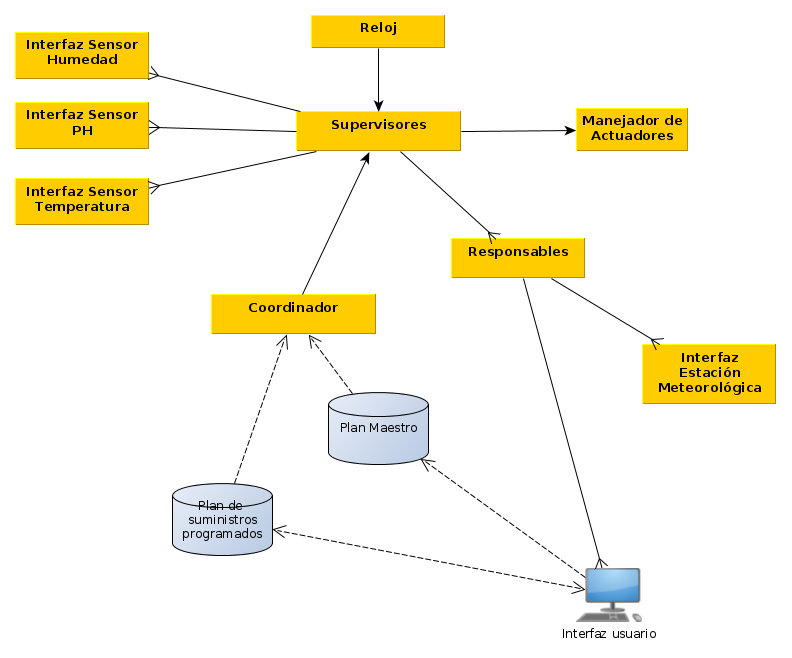
\includegraphics[width=1\textwidth]{./images/arq_tp1.png}
  \caption{Esbozo de la arquitectura resultante de la implementación del TP1}
  \label{fig:comp1}
\end{figure}
De la comparación de las figuras se observa el incremento de complejidad natural al pasar de un entorno controlado y con una sola planta 
a uno con varias plantas distintas, de diferentes tipos y ubicadas en diferentes lugares del país.

En primer lugar observamos que al tener directamente sensores en la tierra no necesitábamos drones para tomar fotos ni componentes para analizar imágenes,
la información sobre el suelo era accesible directamente.

De un modo similar en la comunicación con la interfaz meteorológica evitábamos tener que localizar el lugar de origen de los datos, y nos ahorramos
los componentes específicos para analizar los datos. 

Por otro lado, al haber menor necesidad de guardar información a lo largo del tiempo, hacían falta menos repositorios distribuidos a lo largo de la arquitectura.
El único repositorio de la arquitectura actual que viene de la arquitectura del TP anterior es el de Plan(es) Maestro(s), un concepto que sobrevive todo cambio de
arquitecturas por su importancia en el dominio.
Muchos de los repositorios nuevos que se agregaron tienen que ver con el gran flujo de datos y eventos y la imposibilidad de responder a todos ellos en tiempo real,
algo que en el TP1 no ocurría.

En general vemos que la sucesión de colaboraciones desde la llegada de nueva información hasta el accionar (o no) de los actuadores 
era mucho más simple y corta en el TP1 que en el 2do, presentando componentes con responsabilidades más generales, como los ``Supervisores'' que combina responsabilidades
de que en el TP2 aparecen distribuidas entre la comunicación con los sensores, el analizador de los datos, almacenador, controlador de estadios, planificador, etc.

Sin embargo, si bien las diferencias son variadas y profundas, observamos cierta similitud general entre los diagramas. Algo que podríamos llamar la ``esencia'' de la 
arquitectura permaneció intacto de un TP a otro (aunque casi imposible de visualizar al ojo no entrenado en el dominio del problema). Dicho en términos de la materia,
ambas arquitecturas presentan un estilo similar: existen sensores, el sistema les pide información a esos sensores, la procesa y en función del resultado y de 
lógicas preestablecidas que consulta a partir de repositorios toma decisiones que envía a un conjunto de actuadores que intervienen en el medio de la(s) planta(s).